% this is source code for one of the sessions in Digital Skills for Research Workshop (EMTTI, University of Wolverhampton)
% March 2022, Maria Kunilovskaya (mkunilovskaya@gmail.com)

\documentclass[a4paper,11pt]{article}

\usepackage[utf8]{inputenc}

\usepackage[colorlinks=true, linkcolor=blue, urlcolor=cyan, filecolor=magenta,citecolor=violet]{hyperref} 

\usepackage{geometry}
\geometry{
	a4paper,
	total={170mm,257mm},
	left=20mm,
	top=15mm,
}
\setlength\parindent{0pt} % set all indents to 0
\usepackage{tcolorbox} 
\usepackage{multicol}

\usepackage{listings}
\lstset{basicstyle=\ttfamily\footnotesize}

\makeatletter
\renewcommand*{\verbatim@font}{\ttfamily\footnotesize}
\makeatother

%%% Tables
\usepackage{tabularx,booktabs}
\usepackage{multirow}

%%% Bibliography (makes changes to cite command and at the end of the doc)
%====================
% Switch to biblatex
% intext: \autocite{}, \textcite{knuth1984}, \autocite[\ppno~347--348]{RobertAdams1991}
% references list: \printbibliography[title=Cited]
%====================
%\usepackage[style=authoryear,backend=bibtex]{biblatex}
%\bibliography{7_NLP-tasks-complexity.bib}

%========================
% Use bibtex with natbib
% intext: \citep{}, \citet{}
% references list (at the end of doc): \bibliography{7_NLP-tasks-complexity.bib}
%========================
\usepackage[round,sort,comma]{natbib}

%\usepackage{notoccite} % uncomment to print all items from .bib

\title{Session 6. Bibliographies}
\author{Digital Skills for Research}
\date{March 18, 2022}

\begin{document}
	
\clearpage
\maketitle
\thispagestyle{empty}

\tableofcontents

\section{Intro to referencing styles}

\begin{tcolorbox}[colback=red!5!white, colframe=red!75!black]
	\centering
	{\Large{What is your most used referencing style (APA, Chicago, Harvard)?}}
\end{tcolorbox}
\bigskip
In most cases, the bibliography is taken care of by the template. \\
If not, it helps to know \emph{what you want to see} in the end. 
\bigskip

\begin{itemize}
	\item Referencing (citation) styles are defined by guides (manuals) published by scholarly associations or by publishing companies (e.g. American Psychological Association, University of Chicago or The Institute of Electrical and Electronics Engineers (IEEE))
	\item A referencing style dictates which information about cited works is necessary and how it should be ordered, as well as punctuation and other formatting.
	\item Typically, a citation can include the author's name, date, location of the publishing company, journal title, or DOI (Digital Object Identifer).
	\item There are rules for each type of referred material (book, conference paper, journal article, edited volume)
	\item \textbf{Harvard} has at least 7 (seven!) versions. Consistency matters. 
\end{itemize}

\href{https://www.citethemrightonline.com/Basics}{\underline{The basics of referencing}}

\medskip

Compare entries for a paper published in conference proceedings (\emph{book form}).\\
NB! Book form (not journal form proceedings) are signalled by an ISBN as opposed to  ISSN for journals, by the presence of editors and no volume number.\\
\medskip
Note the use of:
Two columns:
\begin{multicols}{2}
	\begin{itemize}
		\item \verb|&| or `and',
		\item full name or initials for first names,
		\item order of first/last name for $2^d$ author,
		\item brackets for year,
		\item the punctuation to separate blocks of info,
		\item use of quotes and italics,
		\item use of `Eds.' and `pp.'
	\end{itemize}
\end{multicols}

       

\begin{description}
	\item[APA:]	(Shareef et al., 2010), (Elgafy \verb|&| Lafdi, 2010), (Jones, 1998, p. 63)
	
	Shareef, M., Ojo, A., \verb|&| Janowski, T. (2010). Exploring digital divide in the Maldives. In J. Berleur, M. D. Hercheui, \verb|&| L. M. Hilty (Eds.), \textit{What kind of information society? Governance, virtuality, surveillance, sustainability, resilience} (pp. 51–63). Springer. https://doi.org/10.1007/978-3-642-15479-9\_5
	
	\item[\href{https://www.chicagomanualofstyle.org/tools_citationguide/citation-guide-2.html}{Chicago author-year}, \href{https://www.overleaf.com/2121398454pztnvnjshsgk}{Overleaf}:]
	(Singh and Best 1998, 243).
	
	Singh, Kamal, and Gary Best. 2004. ``Film Induced Tourism: Motivations of Visitors to the Hobbiton Movie Set as Featured in `The Lord of the Rings'.'' In \textit{Proceedings of the 1st International Tourism and Media Conference}, Melbourne, 2004, 98-111. Melbourne: Tourism Research Unit, Monash University.
	
	\item[\href{https://www.citethemrightonline.com/comms/conferences/individual-conference-papers}{Harvard}:] (Smith and Jones, 2015, p. 63)
	
	Cook, D. (2014) `Developing franchised business in Scotland', \textit{Small firms: adding the spark: the 23rd ISBA national small firms policy and research conference}. Robert Gordon University, Aberdeen, 15–17 November. Leeds: Institute for Small Business Affairs, pp. 127–136.
	
	\href{https://www.wlv.ac.uk/lib/media/departments/lis/skills/study-guides/LS134-Harvard-Quick-Guide-2018.pdf}{UoW link}
	
\end{description}

\section{\LaTeX~concepts, imports and commands}

\href{https://en.wikibooks.org/wiki/LaTeX/Bibliography_Management}{Bibliography Management}

\subsection{Bibliographic databases}
	
\textbf{Ways to store bibliographic records:}\\

Note unique \textcolor{red}{``citation key''}: lamport94, greenwade93 for each item 

\begin{enumerate}
\item Embedded in the main document
	\begin{lstlisting}
	\usepackage{natbib}
	
	\begin{thebibliography}{9}
	
	\bibitem{lamport94}
	Leslie Lamport,
	\textit{\LaTeX: a document preparation system},
	Addison Wesley, Massachusetts,
	2nd edition,
	1994.
	
	\end{thebibliography}
	\end{lstlisting}

\item Stored in an \href{run:./7_NLP-tasks-complexity.bib}{external .bib file} (e.g. in a BibTex format)

\medskip
\textbf{\textcolor{red}{There are two major formats for these databases: (older) BibTeX and BibLaTex.}}\\
Each format has a dedicated backend, i.e. executable file aka engine to process the database: bibtex and biber, respectively.\\

\newpage


\subsection{General setup for automatic referencing}

\begin{enumerate}
	\item import bibliography manager (natbib) 
	\item specify the stylefile (default or imported from custom .bst)
	\item provide the database (embeded or .bib) and generate References (only cited works) or Bibliography (everything in the file)

\end{enumerate}
	\textcolor{red}{NB!} compatibility between managers, commands and styles can be limited, use recommended combinations

\textbf{A typical entry in a bibtex-style .bib file:}\\

\begin{lstlisting}
	@article{greenwade93,
	author  = "George D. Greenwade",
	title   = "The {C}omprehensive {T}ex {A}rchive {N}etwork ({CTAN})",
	year    = "1993",
	journal = "TUGBoat",
	volume  = "14",
	number  = "3",
	pages   = "342--351"
	}
\end{lstlisting}

\end{enumerate}	

{\Large{\textbf{Setup and Usage}}}

The formats are mutually convertible and compatible, but use different commansa for in-text citations and references list induction.\\


\begin{tcolorbox}[colback=blue!5!white, colframe=blue!85!gray, title=\textbf{Bibtex},center title, toptitle=2mm, bottomtitle=2mm]
	
\begin{multicols}{2}
	
\textbf{Source code}
\begin{lstlisting}
\usepackage[round,sort,comma]{natbib}
...
\begin{document}

\citep{Scarton2018,Tani2022}
\cite[p.~215]{Tani2022}
As shown by~\citet{Scarton2018}, ...

\bibliographystyle{plainnat}
\bibliography{myrefs.bib}

\end{lstlisting}

\break 

\textbf{Compiled doc}
\begin{lstlisting}

(Scarton and Specia 2018; Tani et al. 2022)
(Tani et al. 2022, p. 215)
As shown by Scarton and Specia (2018), ...
\end{lstlisting}
	
\end{multicols}

\end{tcolorbox}

\begin{tcolorbox}[colback=yellow!5!white, coltitle=black, colframe=yellow!65!gray, title=\textbf{BibLaTex}, toptitle=2mm, bottomtitle=2mm, center title]
\begin{multicols}{2}
	
\textbf{Source code}
\begin{lstlisting}
\usepackage[style=authoryear,backend=bibtex]{biblatex}
\bibliography{myrefs.bib}
...
\begin{document}

\autocite{Scarton2018,Tani2022}
\autocite[\ppno~347--348, see also his earlier work]{Tani2022}
As shown by~\textcite{Scarton2018}, ...

\printbibliography[title=Cited Works]

\end{lstlisting}

\break

\textbf{Compiled doc}
\begin{lstlisting}

(Scarton and Specia 2018; Tani et al. 2022)
(Tani et al. 2022, pp. 347-348, and earlier work)
As shown by Scarton and Specia (2018), ...
\end{lstlisting}

\end{multicols}
	
\end{tcolorbox}

\section{Advanced functionality}

\subsection{Possible extentions and options}

\begin{itemize}
	\item output all records in .bib: \verb|\usepackage{notoccite}| + \verb|\nocite{*}|
	\item multiple bibliographies (academic refs and resources, dictionaries in separate lists): see \verb|\usepackage{multibib}|
\end{itemize}


\subsection{Wolves' Harvard in LaTeX}

There are several versions of Harvard style, the differences being small and mainly concern the use of punctuation.

None of the solutions I have seen reproduce exactly what is expected by the University of Wolverhamptopn (it seems): \href{https://www.wlv.ac.uk/lib/media/departments/lis/skills/study-guides/LS134-Harvard-Quick-Guide-2018.pdf}{their examples (no conference papers!)}. Conference papers \href{https://www.citethemrightonline.com/comms/conferences/individual-conference-papers}{here} (as advised by library support)

\bigskip

\textbf{Existing solutions:}

\begin{itemize}
	\item \href{https://www.overleaf.com/project/6227c1c064c39caee9540084}{Overleaf MWE}
	\item \href{https://www.ctan.org/pkg/harvard}{Harvard package} from STAN has 7 *.bst, including agsm, apsr, kluwer, jphysicsB, nederlands. They can be called with:
	
	\begin{lstlisting}
	\usepackage{natbib}
	\bibliographystyle{kluwer}
	\end{lstlisting}
	
	None of them meets the requirements. For example, \verb|agsm| gives comma after year in References and `in' before Proceedings, no comma in-text citations
	
	\item Dr \href{https://github.com/TharinduDR/Thesis/}{Tharindu} uses biblatex and 
	\verb|\autocite| in text.
	\item I tried creating a \href{https://github.com/kunilovskaya/dskills_workshop/tree/main/w3_bibs_beamer/wolves.bst}{wolves specification for Harvard}, by following the discussion \href{https://tex.stackexchange.com/questions/134258/harvard-style-bibliography-with-biblatex-almost-but-not-quite/134264#134264}{here} to edit \verb|apsr| and produce \verb|wolves.bst|. This is the setup I am using:
	
	\begin{lstlisting}
	\usepackage{natbib}
	\usepackage{har2nat}
	\bibliographystyle{wolves}
	\end{lstlisting}
	
\end{itemize}

Check out: \href{https://www.mybib.com/tools/harvard-referencing-generator}{Harvard referencing generator}

\section*{Task 6. Annotated bibliography and revision}
\label{task}
\addcontentsline{toc}{section}{Task 6. Annotated bibliography and revision}

\begin{figure}[h!]
	\centering
	\label{fig:integrate}
	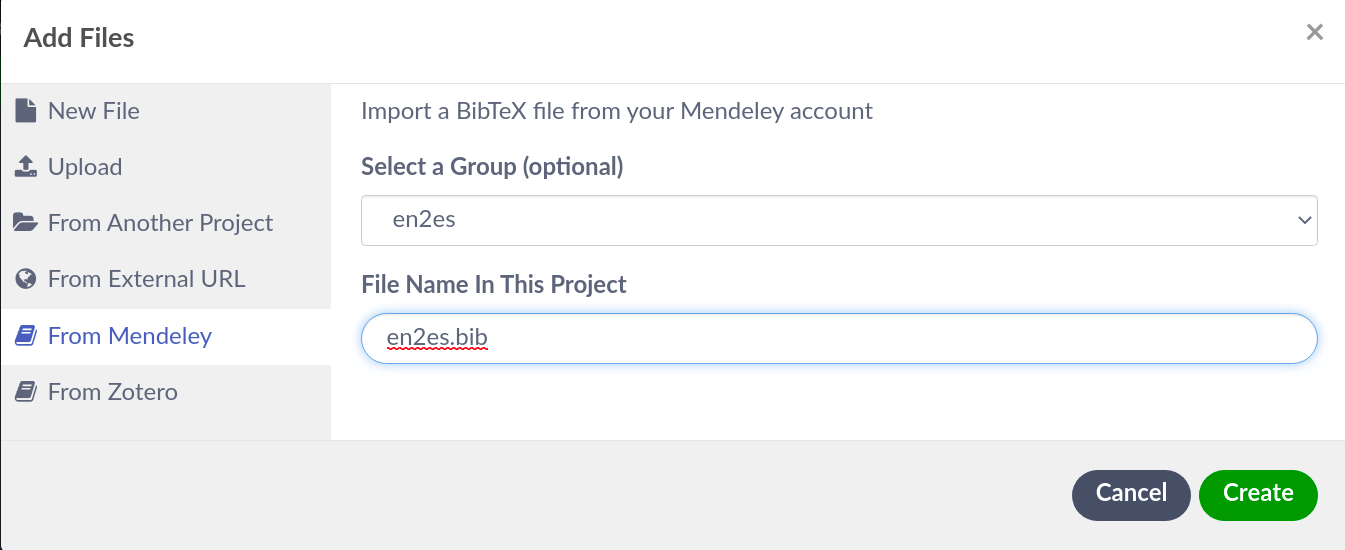
\includegraphics[width=10cm]{pics/group_bib.png}
	\caption{Bib file to Overleaf from the contents of a Mendeley folder}
\end{figure}

\begin{tcolorbox}[width=\textwidth, colback={yellow!40!white}, title={Create an annotated bibliography and revise imported packages}, colbacktitle=yellow!60!white, coltitle=black]
	\begin{enumerate}
		\item As explained \href{https://www.wlv.ac.uk/lib/media/departments/lis/skills/study-guides/LS136-Guide-to-Writing-an-Annotated-Bibliography.pdf}{here}, it is a list of publications with your comments and takeaways.
		
			If you are using Mendeley:
			\begin{itemize}
				\item Link Mendeley account to your Overleaf account
				\item Get bibliographic descriptions of several items you plan to read and put them into a shared folder in Mendeley
				\item Create the project .bib from the folder contents (see Figure~\ref{fig:integrate})
				\item (optional) Can you tweak Mendeley to make use of the field \verb|annote = {These are my take-aways},| which pulls your Notes for the item in Mendeley?
			\end{itemize}
		\item In the source code, which you are encouraged to share with m.kunilovskaya@wlv.ac.uk, use your own words to comment the usage of the packages in the preamble.
	\end{enumerate}
	
\end{tcolorbox}%

Just adding three citeations~\citep{Scarton2018} to generate a short References list~\cite[p.~215]{Tani2022}. This is a citetion intergrated in text:~\citet{Alva-Manchego2021}. 

\bigskip

If you are moving between BibTex and BibLaTex, do delete the temporary files and compile several times before despairing. 


%\nocite{*}

%========================
% If bibtex with natbib
%========================
\bibliographystyle{plainnat}
\bibliography{7_NLP-tasks-complexity.bib}

%========================
% If biblatex
%========================
%\renewcommand*{\bibfont}{\normalsize}
%\renewcommand*{\nameyeardelim}{\addcomma\space}
%\setlength\bibitemsep{10pt}

%\printbibliography[title=Cited Works]


\end{document}